\cotefile{154}
\scanpage{46}
\mspage{1}
Texte français : é, è, ç, à, œ. Une \unsure{lecture|alternative},
\deleted{suppression}, \inserted{addition}, \margin{note marginale},
\illegible{2}, \uline{mot souligné}, \uuline{deux traits}.

\unsure{Un premier paragraphe incertain.

Un deuxième paragraphe avec $\mathscr{A}$ et $\mathfrak{D}$.
\[\unsure{x_i|y_i}=\deleted{a_i}+\inserted{b_i}.\]
Un troisième paragraphe.}

\deleted{Un bloc retiré avec plusieurs paragraphes.

\[\sum_{i=1}^{n}x_i=0.\]
\figure{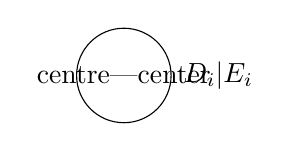
\begin{tikzpicture}[scale=.6]
\draw (0,0) circle (1);\node at (0,0) {\unsure{centre|center}};
\node at (2,0) {$\unsure{D_i|E_i}$};
\end{tikzpicture}}

Un dernier paragraphe retiré.}

\inserted{Un paragraphe ajouté.

\[\bm{v}=\mathbb{R}^{2},\quad\uline{x+y},\quad\uuline{z}.\]
Un deuxième paragraphe ajouté.}

\margin{Une note de marge longue.

Une deuxième ligne de paragraphe avec \illegible{1}.}

\uline{Premier paragraphe souligné.

Deuxième paragraphe souligné.}

\diagram{\begin{tikzcd}
A \arrow[r,"{\unsure{f|g}}"] \arrow[d,hook] & \deleted{B} \\
C \arrow[r,dashed] & D
\end{tikzcd}}

\[\diagram{\begin{array}{cc}a&b\\c&d\end{array}}\]

\deleted{\diagram{\begin{tikzcd}
X \arrow[r,"h"] & Y
\end{tikzcd}}}
